%----------
%	CONFIGURACIÓN DEL DOCUMENTO
%----------
\documentclass[12pt]{report} %fuente a 12pt
% MÁRGENES: 2,5 cm sup. e inf.; 3 cm izdo. y dcho.
\usepackage[
  a4paper,
  vmargin=2.5cm,
  hmargin=3cm
]{geometry}

% INTERLINEADO: Estrecho (6 ptos./interlineado 1,15) o Moderado (6 ptos./interlineado 1,5)
\renewcommand{\baselinestretch}{1.15}
\parskip=6pt

% DEFINICIÓN DE COLORES para portada y listados de código
\usepackage[table]{xcolor}
\definecolor{azulUC3M}{RGB}{0,0,102}
\definecolor{gray97}{gray}{.97}
\definecolor{gray75}{gray}{.75}
\definecolor{gray45}{gray}{.45}

\usepackage[a-1b]{pdfx}
\usepackage{hyperref}

\hypersetup{colorlinks=true,
	linkcolor=black, % enlaces a partes del documento (p.e. índice) en color negro
	urlcolor=blue} % enlaces a recursos fuera del documento en azul

% EXPRESIONES MATEMATICAS
\usepackage{amsmath,amssymb,amsfonts,amsthm}

\usepackage{txfonts}
\usepackage[T1]{fontenc}
\usepackage[utf8]{inputenc}

\usepackage[spanish, es-tabla]{babel}
\usepackage[babel, spanish=spanish]{csquotes}
\AtBeginEnvironment{quote}{\small}

% diseño de PIE DE PÁGINA
\usepackage{fancyhdr}
\pagestyle{fancy}
\fancyhf{}
\renewcommand{\headrulewidth}{0pt}
\rfoot{\thepage}
\fancypagestyle{plain}{\pagestyle{fancy}}

% DISEÑO DE LOS TÍTULOS de las partes del trabajo (capítulos y epígrafes o subcapítulos)
\usepackage{titlesec}
\usepackage{titletoc}
\titleformat{\chapter}[block]
{\large\bfseries\filcenter}
{\thechapter.}
{5pt}
{\MakeUppercase}
{}
\titlespacing{\chapter}{0pt}{0pt}{*3}
\titlecontents{chapter}
[0pt]
{}
{\contentsmargin{0pt}\thecontentslabel.\enspace\uppercase}
{\contentsmargin{0pt}\uppercase}
{\titlerule*[.7pc]{.}\contentspage}

\titleformat{\section}
{\bfseries}
{\thesection.}
{5pt}
{}
\titlecontents{section}
[5pt]
{}
{\contentsmargin{0pt}\thecontentslabel.\enspace}
{\contentsmargin{0pt}}
{\titlerule*[.7pc]{.}\contentspage}

\titleformat{\subsection}
{\normalsize\bfseries}
{\thesubsection.}
{5pt}
{}
\titlecontents{subsection}
[10pt]
{}
{\contentsmargin{0pt}
	\thecontentslabel.\enspace}
{\contentsmargin{0pt}}
{\titlerule*[.7pc]{.}\contentspage}

\usepackage{multirow} % permite combinar celdas
\usepackage{caption} % para personalizar el título de tablas y figuras
\usepackage{floatrow} % utilizamos este paquete y sus macros \ttabbox y \ffigbox para alinear los nombres de tablas y figuras de acuerdo con el estilo definido. Para su uso ver archivo de ejemplo
\usepackage{array} % con este paquete podemos definir en la siguiente línea un nuevo tipo de columna para tablas: ancho personalizado y contenido centrado
\newcolumntype{P}[1]{>{\centering\arraybackslash}p{#1}}
\DeclareCaptionFormat{upper}{#1#2\uppercase{#3}\par}

% Diseño de tabla para ingeniería
\captionsetup[table]{
	format=upper,
	name=TABLA,
	justification=centering,
	labelsep=period,
	width=.75\linewidth,
	labelfont=small,
	font=small,
}

\usepackage{graphicx}
\graphicspath{{imagenes/}} %ruta a la carpeta de imágenes

% Diseño de figuras para ingeniería
\captionsetup[figure]{
	format=hang,
	name=Fig.,
	singlelinecheck=off,
	labelsep=period,
	labelfont=small,
	font=small
}

% NOTAS A PIE DE PÁGINA
\usepackage{chngcntr} %para numeración contínua de las notas al pie
\counterwithout{footnote}{chapter}

% LISTADOS DE CÓDIGO
% soporte y estilo para listados de código. Más información en https://es.wikibooks.org/wiki/Manual_de_LaTeX/Listados_de_código/Listados_con_listings
\usepackage{listings}

% definimos un estilo de listings
\lstdefinestyle{estilo}{ frame=Ltb,
	framerule=0pt,
	aboveskip=0.5cm,
	framextopmargin=3pt,
	framexbottommargin=3pt,
	framexleftmargin=0.4cm,
	framesep=0pt,
	rulesep=.4pt,
	backgroundcolor=\color{gray97},
	rulesepcolor=\color{black},
	%
	basicstyle=\ttfamily\footnotesize,
	keywordstyle=\bfseries,
	stringstyle=\ttfamily,
	showstringspaces = false,
	commentstyle=\color{gray45},
	%
	numbers=left,
	numbersep=15pt,
	numberstyle=\tiny,
	numberfirstline = false,
	breaklines=true,
	xleftmargin=\parindent
}

\captionsetup[lstlisting]{font=small, labelsep=period}
% fijamos el estilo a utilizar
\lstset{style=estilo}
\renewcommand{\lstlistingname}{\uppercase{Código}}


%-------------
%	DOCUMENTO
%-------------

\begin{document}
\pagenumbering{roman} % Se utilizan cifras romanas en la numeración de las páginas previas al cuerpo del trabajo

%----------
%	PORTADA
%----------
\begin{titlepage}
	\begin{sffamily}
	\color{azulUC3M}
	\begin{center}
		\begin{figure}[H] %incluimos el logotipo de la Universidad
			\makebox[\textwidth][c]{
\includegraphics[width=16cm]{Portada_Logo.png}}
		\end{figure}
		\vspace{2.5cm}
		\begin{Large}
			Máster en Ingeniería Informática\\
			2020 - 2021\\
			\vspace{2cm}
			\textsl{Computación de Altas Prestaciones}
			\bigskip

		\end{Large}
		 	{\Huge ``Paralelización de código con OpenMP + MPI''}\\
		 	\vspace*{0.5cm}
	 		\rule{10.5cm}{0.1mm}\\
			\vspace*{0.9cm}
			{\LARGE Carlos Vigil González}\\
            {\LARGE David Gil López}\\
			{\LARGE Daniel Alejandro Rodríguez López}\\
			\vspace*{1cm}
	\end{center}
	\vfill
	\color{black}
	% 
\includegraphics[width=4.2cm]{imagenes/creativecommons.png}\\ %incluimos el logotipo de creativecommons
	% \emph{[Incluir en el caso del interés en su publicación en el archivo abierto]}\\  % BORRAR ESTA LÍNEA
	% Esta obra se encuentra sujeta a la licencia Creative Commons \textbf{Reconocimiento - No Comercial - Sin Obra Derivada}
	\end{sffamily}
\end{titlepage}

%--
% Índice general
%-
\tableofcontents
\thispagestyle{fancy}

%--
% Índice de figuras. Si no se incluyen, comenta las líneas siguientes
%-
\listoffigures
\thispagestyle{fancy}

%--
% Índice de tablas. Si no se incluyen, comenta las líneas siguientes
%-
\listoftables
\thispagestyle{fancy}

%----------
%	TRABAJO
%----------
\clearpage
\pagenumbering{arabic} % numeración con múmeros arábigos para el resto de la publicación

\chapter{Introducción}

La presente memoria explica los pasos seguidos, experimentacón y resultados obtenidos durante la paralelización del código de equalización de histograma entregado inicialmente. Pero antes de entrar en resultados, conviene explicar en qué consiste una equalización de histograma.

De forma simplista, una equalización de histograma consiste en estirar el rango de valores en una imagen para aplanar su histograma de valores.

\begin{figure}[H]
    \makebox[\textwidth][c]{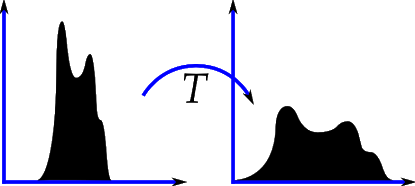
\includegraphics[width=12cm]{histogram_equalization.png}}
    \caption{Ejemplo de Equalización de Histograma}
    \label{fig:hist_eq}
\end{figure}

De forma un poco más técnica, una equalización de histograma distribuye los valores de color en una imagen de forma que todos se encuentran presentes de forma equitativa dentro de la imagen, como se puede apreciar en la \autoref{fig:hist_eq}

Para calcular estos histogramas se debe recorrer la imagen multiples veces, tanto para calcular los valores iniciales como para establecer los valores finales, por lo tanto hemos orientado nuestros esfuerzos con OpenMP(PODRÍAMOS METER REFERENCIA A LA WEB DE OPENMP, PERO NO SE USAR LA BIBLIOGRAFÍA EN LATEX XD) en optimizar estas iteraciones sobre la imagen, mientras que con MPI(MISMO QUE CON OPENMP) nos hemos centrado en el reparto de fragmentos de la imagen entre distintos procesos para reducir el número de iteraciones.

No obstante para poder obtener un análisis más completo de las distintas alternativas y \textit{speed-ups} posibles, se han realizado 3 versiones distintas de paralelización: \nameref{chap:OpenMP}, \nameref{chap:MPI} y \nameref{chap:OpenMP+MPI}. De igual forma, para poder comparar los resultados de forma fiable, se ha utilizado las mismas imágenes de prueba, entorno de ejecución (guernika) y número de ejecuciones.

\section{Análisis}

CARLOS DICE QUE: ESTO CARLOS

Aquí creo que habría que comentar de qué formas hemos visto que es posible paralelizar el código inicial y que partes hacerlas por OpenMP y otras por MPI

\subsection{Speed up teóricos}

El Amdhal inicial y el otro, el que variaba con la carga de trabajo


\chapter{OpenMP}
\label{chap:OpenMP}

Explicar nuestro objetivo con OpenMP y cómo hemos paralelizado cosas

\section{Paralelización}

\section{Experimentación}


\chapter{MPI}
\label{chap:MPI}

Explicar nuestro objetivo con MPI y cómo hemos paralelizado cosas

\section{Paralelización}

\section{Experimentación}


\chapter{OpenMP + MPI}
\label{chap:OpenMP+MPI}
Explicar "conclusiones" o yuqse sobre porqué en base a lo anterior hemos decidido hacer el OpenMP+MPI final, quizás no es exáctamente igual que simplemente juntar lo anterior

\section{Paralelización}

\section{Experimentación}

\chapter{Conclusiones}

Buah colega, hemos aprendido tope mazo

\end{document}
